% Standalone document
\documentclass[notes.tex]{subfiles}
\begin{document}
%%%%%%%%%%%%%%%%%%%%%%%%%%%%%%%%%%%%%%%%%%%%%%%%%%%%%%%
%%%%%%%%%%%%%%%%%%%%%%%%%%%%%%%%%%%%%%%%%%%%%%%%%%%%%%%
\chapter{Breaking supersymmetry}
\label{chap:breaking}
%%%%%%%%%%%%%%%%%%%%%%%%%%%%%%%%%%%%%%%%%%%%%%%%%%%%%%%
%%%%%%%%%%%%%%%%%%%%%%%%%%%%%%%%%%%%%%%%%%%%%%%%%%%%%%%
In Chapter~\ref{chap:poincare} we  saw that  supersymmetry predicts scalar partner particles with the same mass as the known fermions, and new fermions with the same mass as the known vectors, living in the same irreducible representation. These, somewhat unfortunately, contradict experiment by not existing. In this chapter we will look at how we can break supersymmetry so that the new states become more massive, and avoid current experimental bounds. 

%This discussion will be held at a general level, and concrete realisations of this breaking will have to wait until Chapter~\ref{chap:mssm}.


%%%%%%%%%%%%%%%%%%%%%%%%
\section{Spontaneous supersymmetry breaking}
\label{sec:ssb}
%%%%%%%%%%%%%%%%%%%%%%%%
In the Standard Model we have already faced this problem: the vector bosons should remain massless under the gauge symmetry of the model since explicit gauge boson mass terms break the symmetry. Yet, some of them are observed to be very massive indeed. This is solved with the introduction of the Higgs mechanism and {\bf spontaneous symmetry breaking} in the {\bf scalar potential}.\footnote{The potential of the Lagrangian are those terms not containing derivatives of the fields (kinetic terms). The scalar potential are such terms that contain only scalar fields.} The idea is that while there is an internal symmetry of the Lagrangian -- in the Standard Model the gauge symmetry $SU(3)_c\times SU(2)_L\times U(1)_Y$ -- this may not be a symmetry for the particular vacuum state of the theory (the lowest energy state), thereby allowing the properties of the vacuum to supply the masses. In the Standard Model this is achieved by the shape of the scalar potential having a minimum for a non-zero value of the Higgs field which means that the value of the field there -- its {\bf vacuum expectation value} (vev) -- can contribute to the masses. Would it not be great if we could have a similar {\it spontaneous symmetry breaking} in order to break supersymmetry this way and boost the masses of supersymmetric particles beyond current limits?

To find the properties of the vacuum state for our supersymmetric models we start by pointing out that we can write the supersymmetric Hamiltonian as
\[H = \frac{1}{4}(Q_1\bar{Q}_{\dot{1}} + \bar{Q}_{\dot{1}}Q_1 + Q_2\bar{Q}_{\dot{2}} + \bar{Q}_{\dot{2}}Q_2).\]
To see this, consider first
\begin{eqnarray*}
\{Q_A, \bar{Q}_{\dot{B}}\}\bar{\sigma}^{\nu\dot{B}A} &=& 2\sigma^\mu{}_{A\dot{B}}\bar{\sigma}^{\nu\dot{B}A}P_\mu\\
 &=& 2\,{\rm Tr}[\sigma^\mu\bar{\sigma}^\nu]P_\mu\\
  &=& 4g^{\mu\nu}P_\mu =4P^\nu.
\end{eqnarray*}
Now,
\begin{eqnarray*}
H &=& P^0 = \frac{1}{4}\{Q_A, \bar{Q}_{\dot{B}}\} \bar{\sigma}^{0\dot{B}A}\\
 &=& \frac{1}{4}(Q_1\bar{Q}_{\dot{1}} + \bar{Q}_{\dot{1}}Q_1 + Q_2\bar{Q}_{\dot{2}} + \bar{Q}_{\dot{2}}Q_2).
\end{eqnarray*}
As discussed in Section~\ref{sec:weyl} we have $Q_A^\dagger=\bar Q_{\dot A}$. Thus the Hamiltonian is {\bf semipositive definite}, {\it i.e.}\ $\langle H\rangle=\langle \Psi|H|\Psi\rangle \geq 0$ for any state $|\Psi\rangle$, so the energy of any state in supersymmetry is always non-negative.

Imagine now that there exists some lowest lying state (or possibly a set of degenerate states), the ground state(s) $|0\rangle$, that has vanishing energy $\langle0|H|0\rangle = 0$. These states are supersymmetric -- meaning invariant under the supersymmetry transformation -- since, to fulfil the energy assumption, we must have
\begin{equation}
Q_A|0\rangle = \bar{Q}_{\dot{A}}|0\rangle = 0, \quad\text{for all } A,\dot{A},\label{eq:Qvac}
\end{equation}
and are thus invariant under the supersymmetry transformations given by  (\ref{eq:SUSY_trans})
\begin{equation}
\delta_S |0\rangle = (\alpha^AQ_A + \bar{\alpha}_{\dot{A}}\bar{Q}^{\dot{A}})|0\rangle = 0.
\end{equation}
The vanishing energy means that at this supersymmetric minimum of the potential the scalar potential must contribute zero, $\langle V(A, A^*)\rangle=0$, and thus, from Eq.~(\ref{eq:scalarpotglobal}),
\[ \frac{\partial W}{\partial A_i} |0\rangle= 0\quad\text{and} \quad  A_i^*T_{ij}^aA_j|0\rangle=0.\]
Conversely, if the scalar potential does contribute to the energy for the vacuum (ground state) $|0\rangle$, so that it does {\it not} have vanishing energy, meaning that either
\[ \frac{\partial W}{\partial A_i} |0\rangle\neq 0 \quad\text{or}\quad  A_i^*T_{ij}^aA_j|0\rangle\neq 0, \]
in the minimum of the potential for some $A_i$, then {\it supersymmetry must be broken}. As in the Standard Model, the Lagrangian is still (super)symmetric, but $|0\rangle$ is not because (\ref{eq:Qvac}) can no longer hold for all the $Q$s.

The {\bf O'Raifeartaigh model} (1975) \cite{O'Raifeartaigh:1975pr} is an example of a model that spontaneously breaks supersymmetry with three scalar superfields $X$, $Y$, $Z$, and the superpotential
\begin{equation}
W=M YZ+gX(Z^2-m^2),
\end{equation}
where $M$, $g$ and $m$ are real non-zero parameters. The scalar potential is
\begin{eqnarray}
V(A, A^*)&=&\left|\frac{\partial W}{\partial A_X}\right|^2+\left|\frac{\partial W}{\partial A_Y}\right|^2+\left|\frac{\partial W}{\partial A_Z}\right|^2\nonumber\\
&=&|g(A_Z^2-m^2)|^2+|M A_Z|^2 +|MA_Y+2gA_XA_Z|^2,
\end{eqnarray}
which can never be zero because setting $A_Z=0$, which is needed for the second term, gives a non-zero contribution $g^2m^4$ from the first term. Since the expectation value at the minimum that breaks supersymmetry is $\langle0|\frac{\partial W}{\partial A_i}|0\rangle$, and $F_i = -\frac{\partial W^*}{\partial A_i}$, the condition for spontaneous supersymmetry breaking with the O'Raifeartaigh mechanism can be written 
\begin{equation}
\langle F_i \rangle \equiv\langle 0|F_i(x)|0\rangle > 0,
\label{eq:Fbreaking}
\end{equation}
hence it is often given the more generic name {\bf F-term breaking} outside of the specific O'Raifeartaigh model. In general $F$-term breaking it is the vacuum expectation value of the auxiliary field of a scalar superfield that supplies the breaking.

In a gauge theory, a similar mechanism is found by adding the Fayet-Iliopolous term $\mathcal{L}_{FI} \sim 2 kV$ where $V$ is an abelian vector superfield. The vev of the $D(x)$ auxiliary field, $\langle D\rangle=\langle 0|D(x)|0\rangle$, will then create a non-zero scalar potential.\footnote{It is {\it always} the auxiliary fields' fault!} This is called the {\bf Fayet-Iliopolous model}, or {\bf D-term breaking}.



%%%%%%%%%%
\section{Supertrace}
%%%%%%%%%%
Unfortunately, the above does not work in practice if all particles are at a low energy scale. The problem is that at {\it tree level} the {\bf supertrace}, STr, of the mass matrix $\mathcal{M}$, meaning the weighted sum of eigenvalues of the mass matrix of the particles in the model, can be shown to vanish, ${\rm STr}\,\mathcal{M}^2 = 0$ even after spontaneous supersymmetry breaking.\footnote{See Ferrara, Girardello and Palumbo (1979) \cite{Ferrara:1979wa}.}

\df{The {\bf supertrace} is given by
\begin{equation}
\str{\mathcal{M}^2} \equiv \sum_s (-1)^{2s}(2s+1)\,\tr{M_s^2},
\end{equation}
where $\mathcal{M}$ is the complete mass matrix of the Lagrangian, $s$ is the spin of particles and $M_s$ is the mass matrix of all spin-$s$ particles.}

For a theory with only scalar superfields, with two fermionic and two bosonic degrees of freedom each, and with mass matrices $M_{1/2}$ and $M_0$ containing the masses of each type of particle on the diagonal, this means that $\str{\mathcal{M}^2}=\tr{M_0^2 - 2M_{1/2}^2}= 0$. While before spontaneous supersymmetry breaking each fermion and boson in the same superfield had equal masses, we now have that the sum of (the square of) the fermion and boson masses over all the superfields is the same.\footnote{The factor of two takes care of the fact that there is only half as many fermions as bosons.} Since in the Standard Model we have a lot more fermions than scalars, the crucial consequence is that not all the scalar partners can be heavier than our known fermions in order to balance out the supertrace relationship.

Adding vector superfields does not help because the fermions there have spin-1 vector bosons partners, and in the supertrace these contributions get opposite sign, and cancel each other out. This relationship is a tree level relationship, meaning it does not take into account quantum corrections. However, accounting for those and using strong couplings to move the supertrace value away from zero, the effect does not seems to be enough to build a consistent model.

The solution to the supertrace dilemma is to put the spontaneous supersymmetry breaking up at some higher energy scale $\sqrt{\langle F \rangle}$ -- significantly higher than the electroweak scale -- that we do not currently have experimental access to, so that there are also superfields with fermion and boson partners with much higher masses that fulfil the supertrace relationship, and the electroweak scale fermions and bosons become only a small perturbation on it.



%%%%%%%%%%%%%%%%%%%
\section[Soft breaking]{Soft breaking}
%%%%%%%%%%%%%%%%%%%
There are many alternatives in the literature of how we can break supersymmetry spontaneously at a high energy scale. The names of some popular examples that we will return to in the next section are:
\begin{itemize}
\item Planck-scale Mediated Symmetry Breaking (PMSB)
\item Gauge Mediated Symmetry Breaking (GMSB) 
\item Anomaly Mediated Symmetry Breaking (AMSB)
\end{itemize}
Common to all of them is that the mass scale of the particles in the supersymmetry breaking fields is so high, that we can not observe their effects directly. What we can do instead is to parameterise our ignorance by adding effective explicit supersymmetry breaking terms to our low-energy Lagrangian.

However, we cannot simply add arbitrary terms to the Lagrangian. The terms we can add are so-called {\bf soft terms} with couplings of mass dimension one or higher. The dis-allowed terms with smaller mass dimension are terms that can lead to divergences in loop contributions to scalar masses (such as the Higgs) that are quadratic or worse (because of the high dimensionality of the fields in the loops). This will re-introduce the hierarchy problem. 

The allowed terms are in superfield notation as follows:
\begin{eqnarray}
\mathcal{L}_{\rm soft} &=& -\frac{1}{4 T(R)} M \theta\theta\bar{\theta}\bar{\theta} {\rm Tr}\{W^AW_A\} - \frac{1}{6}a_{ijk}\theta\theta\bar{\theta}\bar{\theta} \Phi_i\Phi_j\Phi_k \nonumber\\
&&-\frac{1}{2}b_{ij}\theta\theta\bar{\theta}\bar{\theta} \Phi_i \Phi_j - t_i \theta\theta\bar{\theta}\bar{\theta} \Phi_i +\text{h.c.} \nonumber \\
&& - m_{ij}^2 \theta\theta\bar{\theta}\bar{\theta} \Phi_i^\dagger \Phi_j, \label{eq:gensoftterms}
\end{eqnarray}
where $M,a_{ijk},b_{ij},t_i\in\mathbb C$ and $m_{ij}^2\in\mathbb R$ are the couplings.
Note that these terms are explicitly {\it not} supersymmetric. From the $\theta\theta\bar{\theta}\bar{\theta}$-factors we see that only the lowest order in $\theta$ component fields of the superfields contribute. 

There are also some terms that are called "maybe-soft" terms:
\begin{equation}
\mathcal{L}_{\rm maybe} = -\frac{1}{2} \theta\theta\bar{\theta}\bar{\theta}c_{ijk} \Phi_i^\dagger \Phi_j \Phi_k + {\rm h.c.}
\label{eq:maybesoft}
\end{equation}
with $c_{ijk}\in\mathbb C$. This last -- oft ignored -- type of term is soft as long as none of the scalar superfields is a singlet under all gauge symmetries. It is, however, quite difficult to get large values for $c_{ijk}$ with spontaneous supersymmetry breaking. In the above terms we have not specified any gauge symmetry, which will, in the same way as it did for the superpotential, severely restrict the allowed terms. However, it turns out that soft-terms are responsible for most of the parameters in supersymmetric theories!

We can instead write the soft terms in terms of their component fields as
\begin{eqnarray}
\mathcal{L}_{\rm soft} &=& -\frac{1}{2} M \lambda^A\lambda_A -(\frac{1}{6}a_{ijk}A_iA_jA_k + \frac{1}{2}b_{ij}A_iA_j + t_i A_i +\frac{1}{2}c_{ijk}A^*_iA_jA_k+\text{c.c.}) \nonumber\\
&& - m_{ij}^2 A_i^*A_j.
\label{eq:soft_terms_component_fields}
\end{eqnarray}
Here we clearly see that the $m_{ij}$ couplings provide extra mass terms to the scalar partners $A_i$ of the fermions in the scalar superfields, and $M$ to the fermion partners $\lambda_A$ of the vectors in the vector superfields. Thus, they split the masses of the partners as we wanted to achieve with breaking supersymmetry.

Now, what happens to the hierarchy problem? Restricting ourselves to soft supersymmetry breaking terms guarantees that we end up with contributions to the Higgs mass of at most
\begin{equation}
\Delta m_h^2 = -\frac{\lambda_s}{16\pi^2}m_s^2\ln\frac{\Lambda_{UV}^2}{m_s^2}+\ldots,
\label{eq:higgs_soft_mass}
\end{equation}
at the leading order in $\Lambda_{UV}$, where $m_s$ is the mass scale of the soft term. The correction to the Higgs mass is thus proportional to the masses of the supersymmetric particles. 

This is the most important argument in favour of supersymmetry existing at low energy scales where we can detect it, because $m_s$ can not be too large if we want the above corrections to be reasonably small. This is called the {\bf little hierarchy problem}, and numerically, given that $16\pi^2\sim 100$, and the couplings $\lambda_s$ are not expected to be above unity,  this means that we want $m_s \sim {\mathcal O}(1~{\rm TeV})$ in order to keep the cancellations reasonable and of the order of the measured Higgs mass, with little fine-tuning.


%%%%%%%%%%%%%%%%%%%%%%%
\section{Models for supersymmetry breaking} 
%%%%%%%%%%%%%%%%%%%%%%%
Let us begin by taking a closer look at the models we use to motivate supersymmetry breaking, and what their phenomenological consequences are. This is important to keep in mind as most searches for supersymmetry are interpreted under certain assumptions on the supersymmetry  breaking mechanism.

Generically such models can be illustrated as shown in Fig.~\ref{SSB}. There is one or more {\bf hidden sector} (HS) scalar superfield $X$ -- by hidden we mean that it has no or very small direct couplings to the MSSM fields -- that has an {\it effective (non-renormalizable) coupling} to the MSSM scalar fields $\Phi_i$ of the form
\begin{equation}
\mathcal{L}_\text{HS} = -\frac{1}{M}(\bar\theta\bar\theta)X\Phi_i\Phi_j\Phi_k,
\label{eq:HS_MSSM}
\end{equation}
where $M$ is some large scale, {\it e.g.}\ the Planck scale, that suppresses the interaction. Figure \ref{SUSYB} shows interactions that can lead to such terms, where $M$ is the mass scale of some {\bf mediator} particle $Y$. 

\begin{figure}[h!]
\centering
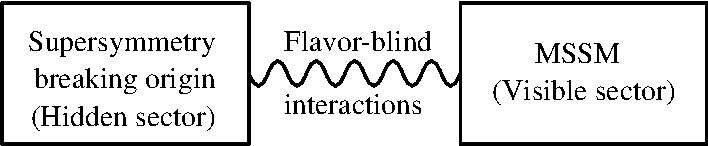
\includegraphics[scale=1.0]{figures/structure} 
\caption{A generic illustration of how to generate soft breaking terms~\cite{Martin:1997ns}. \label{SSB}}
\end{figure}

\begin{figure}[h!]
\begin{center}
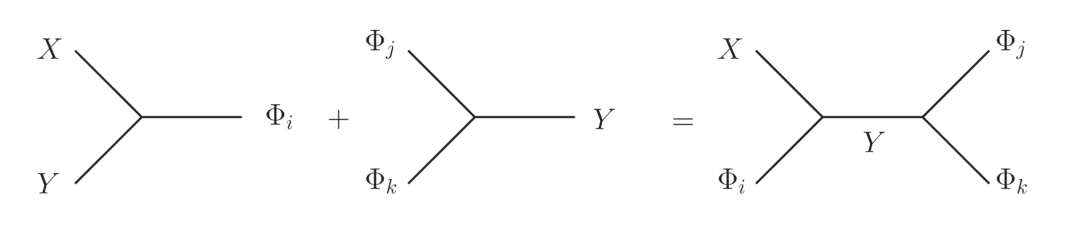
\includegraphics[scale=0.9]{figures/SUSYB} 
\caption{Interactions leading to effective 4-particle couplings in our example. \label{SUSYB}}
\end{center}
\end{figure}

If the hidden sector is constructed so that $X$ develops a vev for its auxillary $F$-component field, $F_X$,\begin{equation}
\langle X \rangle = \theta \theta \langle F_X \rangle,
\end{equation}
it breaks supersymmetry spontaneously, see the discussion leading up to Eq.~(\ref{eq:Fbreaking}). As a result, the interaction in  (\ref{eq:HS_MSSM}) will produce a soft-term of the form of the second term in Eq.~(\ref{eq:soft_terms_component_fields}),
\begin{equation}
\mathcal{L}_\text{soft}=-\frac{\langle F_X \rangle}{M}A_iA_jA_k,
\end{equation}
with the soft-mass parameter
\[m_\text{soft} = \frac{\langle F_X \rangle}{M}.\]
This has reasonable limits in that $m_\text{soft}  \to 0$ as $\langle F_X \rangle \to 0$, which is the limit of no supersymmetry breaking, and $m_{\rm soft} \to 0$ as $M \to \infty$, where the interaction with the hidden sector is decoupled because the mediating particle $Y$ becomes too heavy to have any influence. 

We will now look at two possible ways to construct such a hidden sector called Planck-scale Mediated Supersymmetry Breaking (PMSB) and Gauge Mediated Supersymmetry Breaking (GMSB).


%%%
\subsection{Planck-scale Mediated Supersymmetry Breaking (PMSB)}
%%%
In Planck-scale mediated supersymmetry breaking (PMSB) we blame some gravity mechanism for mediating the supersymmetry breaking from the hidden sector to the MSSM so that the scale of the breaking is $M = M_P = 2.4 \cdot 10^{18}$\,GeV. Then we need to have $\sqrt{\langle F_X\rangle} \sim 10^{10}-10^{11}$\,GeV in order to get $m_{\rm soft} \simeq 50-5000$\,GeV, which is roughly of the right magnitude not to re-introduce the hierarchy problem. The use of $\sqrt{\langle F_X\rangle}$ is just a conventional shorthand notation for the magnitude of the vev of whichever $F$-term that breaks supersymmetry. This is called the {\bf supersymmetry breaking scale}.

The complete soft terms for such a mechanism can then be shown to be
\begin{eqnarray}
\mathcal{L}_\text{soft} &=& -\frac{\langle F_X \rangle}{M_P}\left(\frac{1}{2} f_i \lambda^a_i \lambda^a_i + \frac{1}{6} y'_{ijk}A_i A_j A_k + \frac{1}{2}\mu'_{ij}A_iA_j + \frac{\langle F_X \rangle^*}{M_P^2}x_{ijk}A_i^*A_jA_k + {\rm c.c.}\right)\nonumber\\
 &&- \frac{|\langle F_X \rangle |^2}{M_P^2}k_{ij}A_iA_j^*.
 \end{eqnarray}
Incidentally, we can now see why we assumed the maybe-soft breaking terms to be unimportant, as  in this model they are suppressed by $|\langle F_X \rangle|/M_P^2$ compared to the other masses. 

If one assumes a minimal form for the parameters at the GUT scale, motivated by the wish for unification, {\it e.g.}\ $f_i=f$, $y'_{ijk} = \alpha y_{ijk}$, $\mu'_{ij} = \beta \mu$, and $k_{ij} = k\delta_{ij}$, then all the soft terms are fixed by just four parameters
\[m_{1/2} = f\frac{\langle F_X \rangle}{M_P}, \indent m_0^2 = k \frac{|\langle F_X \rangle|^2}{M_P^2}, \indent A_0 = \alpha \frac{\langle F_X \rangle }{M_P}, \indent B_0 = \beta\frac{\langle F_X \rangle}{M_P}.\]
The resulting phenomenology is called {\bf minimal supergravity}, or {\bf mSUGRA/CMSSM}. This is minimal in the sense of the form of the parameters, and is the most studied, but perhaps not best motivated, version of the MSSM. Usually, $B_0$ and $|\mu|$ are exchanged for $\tan\beta$ at low scales using the EWSB condition  in Eq.~(\ref{eq:EWSB_condition}), so it is common to say that there are four and a half parameters in the model: $m_{1/2}$, $m_0$, $A_0$, $\tan\beta$ and ${\rm sgn}\,\mu$.


%%%
\subsection{Gauge Mediated Supersymmetry Breaking (GMSB)} 
%%%
An alternative to PMSB is gauge-mediated supersymmetry breaking where soft terms come from {\it loop diagrams} with {\bf messenger} superfields that get their own mass by coupling to the hidden sector supersymmetry breaking  vev, and that have Standard Model gauge interactions. By dimensional analysis we must have
\[m_{\rm soft} = \frac{\alpha_i}{4\pi}\frac{\langle F \rangle}{M}.\]
If now the supersymmetry breaking scale  $\sqrt{\langle F\rangle}$ and the messenger mass $M$ are roughly comparable in size, which is reasonable given where the messenger mass comes from, then $\sqrt{\langle F \rangle} \simeq 100$\,TeV can give a viable sparticle spectrum. Notice that there is now a lot less RGE running for the parameters in the GMSB compared to the PMSB since the soft masses are created at a rather low scale.

One way of thinking about how these mass terms appear is that the messenger field(s) get masses from hidden sector vevs and contribute to for example gaugino mass terms through diagrams such as the one in Fig.~\ref{fig:GMSB}, where messenger scalars and fermions run in the loop, and their masses from the hidden sector vevs are symbolised by the mass insertions. Note that scalars can only get mass contributions like this at two-loop order since the messenger interaction is a gauge interaction, involving gauge bosons or gauginos in the MSSM. In order not to spoil GUT unification messengers are often assumed to have small mass splittings and come in $N_5$ complete $\mathbf{5} + \overline{\mathbf{5}}$ (fundamental) representations of $SU(5)$.

\begin{figure}[h!]
\begin{center}
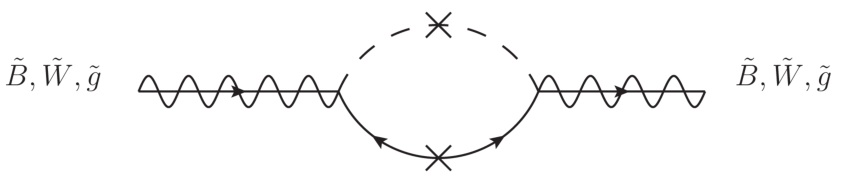
\includegraphics[scale=0.8]{figures/GMSB} 
\caption{Diagram for GMSB giving masses to the gauginos. The messenger scalars and fermions run in the loop.}
\label{fig:GMSB}
\end{center}
\end{figure}

The minimal parametrisation of GMSB models is in terms of the scale $\Lambda = \frac{\langle F\rangle}{M}$, the messenger mass $M$, the number of representations $N_5$, and $\tan\beta$ for the EWSB criterion (instead of $\mu$ and $b$). This gives the soft masses
\begin{eqnarray}
M_i &=& \frac{\alpha_i}{4\pi}\Lambda N_5,\quad\text{(gaugino masses)}\label{eq:GMSBgauginomass}\\
m_j^2 &=& 2\Lambda^2 N_5 \sum C(R)_i\left(\frac{\alpha_i}{4\pi}\right)^2,\quad\text{(scalar masses)}
\end{eqnarray}
where the sum is over the quadratic Casimir invariant for the scalar superfield $\Phi_j$ that the scalar field belongs to. We clearly see that the scalar soft-masses are a two-loop effect as discussed above. 

While this parameterisation looks independent of $M$, the messenger scale sets the starting point of the RGE running of the sparticle masses, and thus influences their magnitude. For example, the tri-linear soft-term couplings $a_{ijk}$ are expected to be very small at the messenger scale, and are effectively set to zero, however, due to RGE running they are small, but non-zero at the electroweak scale. Since the scalar masses $m_j$ scale as $\sqrt{N_5}$ compared to $N_5$ for the gauginos, we in general expect the scalars to be lighter in GMSB models. One should also notice that this parameterisation  gives the same hierarchy of gaugino masses as in mSUGRA, $M_3>M_2>M_1$, since (\ref{eq:GMSBgauginomass}) is ordered in terms of the strength of the gauge couplings $\alpha_i$. The origin of the hierarchy is different since in mSUGRA it comes from the running of the parameters down from the GUT scale.





%%%%%%%%%%%%%
\section{Excercises}
%%%%%%%%%%%%%

\begin{Exercise}[]
Show that adding a Fayet-Iliopolous term to the SQED constructed in Exercise \ref{chap:lagrangian}.\ref{ex:SQED} will break supersymmetry spontaneously.
\end{Exercise}

\begin{Exercise}[]
Write down the supertrace relationship for a spontaneously broken SQED.
\end{Exercise}



\end{document}


